% REV01 Sun 27 Jun 2021 14:17:49 WIB
% START Tue 04 May 2021 13:55:16 WIB

\chapter{WHAT WAS CAUGHT IN THE TRAPS THAT WERE SET}

How Bradley Headstone had been racked and riven in his mind since the
quiet evening when by the river-side he had risen, as it were, out of
the ashes of the Bargeman, none but he could have told. Not even he
could have told, for such misery can only be felt.

First, he had to bear the combined weight of the knowledge of what he
had done, of that haunting reproach that he might have done it so much
better, and of the dread of discovery. This was load enough to crush
him, and he laboured under it day and night. It was as heavy on him in
his scanty sleep, as in his red-eyed waking hours. It bore him down with
a dread unchanging monotony, in which there was not a moment’s variety.
The overweighted beast of burden, or the overweighted slave, can for
certain instants shift the physical load, and find some slight respite
even in enforcing additional pain upon such a set of muscles or such
a limb. Not even that poor mockery of relief could the wretched man
obtain, under the steady pressure of the infernal atmosphere into which
he had entered.

Time went by, and no visible suspicion dogged him; time went by, and
in such public accounts of the attack as were renewed at intervals,
he began to see Mr Lightwood (who acted as lawyer for the injured man)
straying further from the fact, going wider of the issue, and evidently
slackening in his zeal. By degrees, a glimmering of the cause of this
began to break on Bradley’s sight. Then came the chance meeting with Mr
Milvey at the railway station (where he often lingered in his leisure
hours, as a place where any fresh news of his deed would be circulated,
or any placard referring to it would be posted), and then he saw in the
light what he had brought about.

For, then he saw that through his desperate attempt to separate those
two for ever, he had been made the means of uniting them. That he had
dipped his hands in blood, to mark himself a miserable fool and tool.
That Eugene Wrayburn, for his wife’s sake, set him aside and left him to
crawl along his blasted course. He thought of Fate, or Providence, or
be the directing Power what it might, as having put a fraud upon
him--overreached him--and in his impotent mad rage bit, and tore, and
had his fit.

New assurance of the truth came upon him in the next few following days,
when it was put forth how the wounded man had been married on his bed,
and to whom, and how, though always in a dangerous condition, he was a
shade better. Bradley would far rather have been seized for his murder,
than he would have read that passage, knowing himself spared, and
knowing why.

But, not to be still further defrauded and overreached--which he would
be, if implicated by Riderhood, and punished by the law for his abject
failure, as though it had been a success--he kept close in his school
during the day, ventured out warily at night, and went no more to the
railway station. He examined the advertisements in the newspapers for
any sign that Riderhood acted on his hinted threat of so summoning him
to renew their acquaintance, but found none. Having paid him handsomely
for the support and accommodation he had had at the Lock House, and
knowing him to be a very ignorant man who could not write, he began to
doubt whether he was to be feared at all, or whether they need ever meet
again.

All this time, his mind was never off the rack, and his raging sense of
having been made to fling himself across the chasm which divided those
two, and bridge it over for their coming together, never cooled down.
This horrible condition brought on other fits. He could not have said
how many, or when; but he saw in the faces of his pupils that they had
seen him in that state, and that they were possessed by a dread of his
relapsing.

One winter day when a slight fall of snow was feathering the sills and
frames of the schoolroom windows, he stood at his black board, crayon in
hand, about to commence with a class; when, reading in the countenances
of those boys that there was something wrong, and that they seemed in
alarm for him, he turned his eyes to the door towards which they faced.
He then saw a slouching man of forbidding appearance standing in the
midst of the school, with a bundle under his arm; and saw that it was
Riderhood.

He sat down on a stool which one of his boys put for him, and he had a
passing knowledge that he was in danger of falling, and that his face
was becoming distorted. But, the fit went off for that time, and he
wiped his mouth, and stood up again.

‘Beg your pardon, governor! By your leave!’ said Riderhood, knuckling
his forehead, with a chuckle and a leer. ‘What place may this be?’

‘This is a school.’

‘Where young folks learns wot’s right?’ said Riderhood, gravely nodding.
‘Beg your pardon, governor! By your leave! But who teaches this school?’

‘I do.’

‘You’re the master, are you, learned governor?’

‘Yes. I am the master.’

‘And a lovely thing it must be,’ said Riderhood, ‘fur to learn young
folks wot’s right, and fur to know wot THEY know wot you do it. Beg your
pardon, learned governor! By your leave!--That there black board; wot’s
it for?’

‘It is for drawing on, or writing on.’

‘Is it though!’ said Riderhood. ‘Who’d have thought it, from the
looks on it! WOULD you be so kind as write your name upon it, learned
governor?’ (In a wheedling tone.)

Bradley hesitated for a moment; but placed his usual signature,
enlarged, upon the board.

‘I ain’t a learned character myself,’ said Riderhood, surveying the
class, ‘but I do admire learning in others. I should dearly like to hear
these here young folks read that there name off, from the writing.’

The arms of the class went up. At the miserable master’s nod, the shrill
chorus arose: ‘Bradley Headstone!’

‘No?’ cried Riderhood. ‘You don’t mean it? Headstone! Why, that’s in a
churchyard. Hooroar for another turn!’

Another tossing of arms, another nod, and another shrill chorus:

‘Bradley Headstone!’

‘I’ve got it now!’ said Riderhood, after attentively listening, and
internally repeating: ‘Bradley. I see. Chris’en name, Bradley sim’lar to
Roger which is my own. Eh? Fam’ly name, Headstone, sim’lar to Riderhood
which is my own. Eh?’

Shrill chorus. ‘Yes!’

‘Might you be acquainted, learned governor,’ said Riderhood, ‘with a
person of about your own heighth and breadth, and wot ‘ud pull down in
a scale about your own weight, answering to a name sounding summat like
Totherest?’

With a desperation in him that made him perfectly quiet, though his jaw
was heavily squared; with his eyes upon Riderhood; and with traces of
quickened breathing in his nostrils; the schoolmaster replied, in a
suppressed voice, after a pause: ‘I think I know the man you mean.’

‘I thought you knowed the man I mean, learned governor. I want the man.’

With a half glance around him at his pupils, Bradley returned:

‘Do you suppose he is here?’

‘Begging your pardon, learned governor, and by your leave,’ said
Riderhood, with a laugh, ‘how could I suppose he’s here, when there’s
nobody here but you, and me, and these young lambs wot you’re a learning
on? But he is most excellent company, that man, and I want him to come
and see me at my Lock, up the river.’

‘I’ll tell him so.’

‘D’ye think he’ll come?’ asked Riderhood.

‘I am sure he will.’

‘Having got your word for him,’ said Riderhood, ‘I shall count upon him.
P’raps you’d so fur obleege me, learned governor, as tell him that if he
don’t come precious soon, I’ll look him up.’

‘He shall know it.’

‘Thankee. As I says a while ago,’ pursued Riderhood, changing his hoarse
tone and leering round upon the class again, ‘though not a learned
character my own self, I do admire learning in others, to be sure! Being
here and having met with your kind attention, Master, might I, afore I
go, ask a question of these here young lambs of yourn?’

‘If it is in the way of school,’ said Bradley, always sustaining his
dark look at the other, and speaking in his suppressed voice, ‘you may.’

‘Oh! It’s in the way of school!’ cried Riderhood. ‘I’ll pound it,
Master, to be in the way of school. Wot’s the diwisions of water, my
lambs? Wot sorts of water is there on the land?’

Shrill chorus: ‘Seas, rivers, lakes, and ponds.’

‘Seas, rivers, lakes, and ponds,’ said Riderhood. ‘They’ve got all the
lot, Master! Blowed if I shouldn’t have left out lakes, never having
clapped eyes upon one, to my knowledge. Seas, rivers, lakes, and ponds.
Wot is it, lambs, as they ketches in seas, rivers, lakes, and ponds?’

Shrill chorus (with some contempt for the ease of the question):

‘Fish!’

‘Good a-gin!’ said Riderhood. ‘But wot else is it, my lambs, as they
sometimes ketches in rivers?’

Chorus at a loss. One shrill voice: ‘Weed!’

‘Good agin!’ cried Riderhood. ‘But it ain’t weed neither. You’ll never
guess, my dears. Wot is it, besides fish, as they sometimes ketches in
rivers? Well! I’ll tell you. It’s suits o’ clothes.’

Bradley’s face changed.

‘Leastways, lambs,’ said Riderhood, observing him out of the corners
of his eyes, ‘that’s wot I my own self sometimes ketches in rivers. For
strike me blind, my lambs, if I didn’t ketch in a river the wery bundle
under my arm!’

The class looked at the master, as if appealing from the irregular
entrapment of this mode of examination. The master looked at the
examiner, as if he would have torn him to pieces.

‘I ask your pardon, learned governor,’ said Riderhood, smearing his
sleeve across his mouth as he laughed with a relish, ‘tain’t fair to the
lambs, I know. It wos a bit of fun of mine. But upon my soul I drawed
this here bundle out of a river! It’s a Bargeman’s suit of clothes. You
see, it had been sunk there by the man as wore it, and I got it up.’

‘How do you know it was sunk by the man who wore it?’ asked Bradley.

‘Cause I see him do it,’ said Riderhood.

They looked at each other. Bradley, slowly withdrawing his eyes, turned
his face to the black board and slowly wiped his name out.

‘A heap of thanks, Master,’ said Riderhood, ‘for bestowing so much of
your time, and of the lambses’ time, upon a man as hasn’t got no other
recommendation to you than being a honest man. Wishing to see at my Lock
up the river, the person as we’ve spoke of, and as you’ve answered for,
I takes my leave of the lambs and of their learned governor both.’

With those words, he slouched out of the school, leaving the master
to get through his weary work as he might, and leaving the whispering
pupils to observe the master’s face until he fell into the fit which had
been long impending.

The next day but one was Saturday, and a holiday. Bradley rose early,
and set out on foot for Plashwater Weir Mill Lock. He rose so early that
it was not yet light when he began his journey. Before extinguishing the
candle by which he had dressed himself, he made a little parcel of his
decent silver watch and its decent guard, and wrote inside the paper:
‘Kindly take care of these for me.’ He then addressed the parcel to Miss
Peecher, and left it on the most protected corner of the little seat in
her little porch.

It was a cold hard easterly morning when he latched the garden gate
and turned away. The light snowfall which had feathered his schoolroom
windows on the Thursday, still lingered in the air, and was falling
white, while the wind blew black. The tardy day did not appear until he
had been on foot two hours, and had traversed a greater part of London
from east to west. Such breakfast as he had, he took at the comfortless
public-house where he had parted from Riderhood on the occasion of
their night-walk. He took it, standing at the littered bar, and looked
loweringly at a man who stood where Riderhood had stood that early
morning.

He outwalked the short day, and was on the towing-path by the river,
somewhat footsore, when the night closed in. Still two or three miles
short of the Lock, he slackened his pace then, but went steadily on. The
ground was now covered with snow, though thinly, and there were floating
lumps of ice in the more exposed parts of the river, and broken sheets
of ice under the shelter of the banks. He took heed of nothing but the
ice, the snow, and the distance, until he saw a light ahead, which he
knew gleamed from the Lock House window. It arrested his steps, and he
looked all around. The ice, and the snow, and he, and the one light, had
absolute possession of the dreary scene. In the distance before him, lay
the place where he had struck the worse than useless blows that mocked
him with Lizzie’s presence there as Eugene’s wife. In the distance
behind him, lay the place where the children with pointing arms had
seemed to devote him to the demons in crying out his name. Within there,
where the light was, was the man who as to both distances could give him
up to ruin. To these limits had his world shrunk.

He mended his pace, keeping his eyes upon the light with a strange
intensity, as if he were taking aim at it. When he approached it so
nearly as that it parted into rays, they seemed to fasten themselves
to him and draw him on. When he struck the door with his hand, his foot
followed so quickly on his hand, that he was in the room before he was
bidden to enter.

The light was the joint product of a fire and a candle. Between the two,
with his feet on the iron fender, sat Riderhood, pipe in mouth.

He looked up with a surly nod when his visitor came in. His visitor
looked down with a surly nod. His outer clothing removed, the visitor
then took a seat on the opposite side of the fire.

‘Not a smoker, I think?’ said Riderhood, pushing a bottle to him across
the table.

‘No.’

They both lapsed into silence, with their eyes upon the fire.

‘You don’t need to be told I am here,’ said Bradley at length. ‘Who is
to begin?’

‘I’ll begin,’ said Riderhood, ‘when I’ve smoked this here pipe out.’

He finished it with great deliberation, knocked out the ashes on the
hob, and put it by.

‘I’ll begin,’ he then repeated, ‘Bradley Headstone, Master, if you wish
it.’

‘Wish it? I wish to know what you want with me.’

‘And so you shall.’ Riderhood had looked hard at his hands and his
pockets, apparently as a precautionary measure lest he should have any
weapon about him. But, he now leaned forward, turning the collar of
his waistcoat with an inquisitive finger, and asked, ‘Why, where’s your
watch?’

‘I have left it behind.’

‘I want it. But it can be fetched. I’ve took a fancy to it.’

Bradley answered with a contemptuous laugh.

‘I want it,’ repeated Riderhood, in a louder voice, ‘and I mean to have
it.’

‘That is what you want of me, is it?’

‘No,’ said Riderhood, still louder; ‘it’s on’y part of what I want of
you. I want money of you.’

‘Anything else?’

‘Everythink else!’ roared Riderhood, in a very loud and furious way.
‘Answer me like that, and I won’t talk to you at all.’

Bradley looked at him.

‘Don’t so much as look at me like that, or I won’t talk to you at all,’
vociferated Riderhood. ‘But, instead of talking, I’ll bring my hand
down upon you with all its weight,’ heavily smiting the table with great
force, ‘and smash you!’

‘Go on,’ said Bradley, after moistening his lips.

‘O! I’m a going on. Don’t you fear but I’ll go on full-fast enough for
you, and fur enough for you, without your telling. Look here, Bradley
Headstone, Master. You might have split the T’other governor to chips
and wedges, without my caring, except that I might have come upon you
for a glass or so now and then. Else why have to do with you at all? But
when you copied my clothes, and when you copied my neckhankercher, and
when you shook blood upon me after you had done the trick, you did wot
I’ll be paid for and paid heavy for. If it come to be throw’d upon you,
you was to be ready to throw it upon me, was you? Where else but
in Plashwater Weir Mill Lock was there a man dressed according as
described? Where else but in Plashwater Weir Mill Lock was there a
man as had had words with him coming through in his boat? Look at the
Lock-keeper in Plashwater Weir Mill Lock, in them same answering clothes
and with that same answering red neckhankercher, and see whether his
clothes happens to be bloody or not. Yes, they do happen to be bloody.
Ah, you sly devil!’

Bradley, very white, sat looking at him in silence.

‘But two could play at your game,’ said Riderhood, snapping his fingers
at him half a dozen times, ‘and I played it long ago; long afore you
tried your clumsy hand at it; in days when you hadn’t begun croaking
your lecters or what not in your school. I know to a figure how you
done it. Where you stole away, I could steal away arter you, and do it
knowinger than you. I know how you come away from London in your own
clothes, and where you changed your clothes, and hid your clothes. I see
you with my own eyes take your own clothes from their hiding-place
among them felled trees, and take a dip in the river to account for
your dressing yourself, to any one as might come by. I see you rise up
Bradley Headstone, Master, where you sat down Bargeman. I see you pitch
your Bargeman’s bundle into the river. I hooked your Bargeman’s bundle
out of the river. I’ve got your Bargeman’s clothes, tore this way and
that way with the scuffle, stained green with the grass, and spattered
all over with what bust from the blows. I’ve got them, and I’ve got you.
I don’t care a curse for the T’other governor, alive or dead, but I care
a many curses for my own self. And as you laid your plots agin me and
was a sly devil agin me, I’ll be paid for it--I’ll be paid for it--I’ll
be paid for it--till I’ve drained you dry!’

Bradley looked at the fire, with a working face, and was silent for a
while. At last he said, with what seemed an inconsistent composure of
voice and feature:

‘You can’t get blood out of a stone, Riderhood.’

‘I can get money out of a schoolmaster though.’

‘You can’t get out of me what is not in me. You can’t wrest from me what
I have not got. Mine is but a poor calling. You have had more than two
guineas from me, already. Do you know how long it has taken me (allowing
for a long and arduous training) to earn such a sum?’

‘I don’t know, nor I don’t care. Yours is a ‘spectable calling. To
save your ‘spectability, it’s worth your while to pawn every article of
clothes you’ve got, sell every stick in your house, and beg and borrow
every penny you can get trusted with. When you’ve done that and handed
over, I’ll leave you. Not afore.’

‘How do you mean, you’ll leave me?’

‘I mean as I’ll keep you company, wherever you go, when you go away from
here. Let the Lock take care of itself. I’ll take care of you, once I’ve
got you.’

Bradley again looked at the fire. Eyeing him aside, Riderhood took up
his pipe, refilled it, lighted it, and sat smoking. Bradley leaned his
elbows on his knees, and his head upon his hands, and looked at the fire
with a most intent abstraction.

‘Riderhood,’ he said, raising himself in his chair, after a long
silence, and drawing out his purse and putting it on the table. ‘Say
I part with this, which is all the money I have; say I let you have
my watch; say that every quarter, when I draw my salary, I pay you a
certain portion of it.’

‘Say nothink of the sort,’ retorted Riderhood, shaking his head as he
smoked. ‘You’ve got away once, and I won’t run the chance agin. I’ve had
trouble enough to find you, and shouldn’t have found you, if I hadn’t
seen you slipping along the street overnight, and watched you till you
was safe housed. I’ll have one settlement with you for good and all.’

‘Riderhood, I am a man who has lived a retired life. I have no resources
beyond myself. I have absolutely no friends.’

‘That’s a lie,’ said Riderhood. ‘You’ve got one friend as I knows of;
one as is good for a Savings-Bank book, or I’m a blue monkey!’

Bradley’s face darkened, and his hand slowly closed on the purse and
drew it back, as he sat listening for what the other should go on to
say.

‘I went into the wrong shop, fust, last Thursday,’ said Riderhood.
‘Found myself among the young ladies, by George! Over the young ladies,
I see a Missis. That Missis is sweet enough upon you, Master, to sell
herself up, slap, to get you out of trouble. Make her do it then.’

Bradley stared at him so very suddenly that Riderhood, not quite knowing
how to take it, affected to be occupied with the encircling smoke from
his pipe; fanning it away with his hand, and blowing it off.

‘You spoke to the mistress, did you?’ inquired Bradley, with that
former composure of voice and feature that seemed inconsistent, and with
averted eyes.

‘Poof! Yes,’ said Riderhood, withdrawing his attention from the smoke.
‘I spoke to her. I didn’t say much to her. She was put in a fluster by
my dropping in among the young ladies (I never did set up for a lady’s
man), and she took me into her parlour to hope as there was nothink
wrong. I tells her, “O no, nothink wrong. The master’s my wery good
friend.” But I see how the land laid, and that she was comfortable off.’

Bradley put the purse in his pocket, grasped his left wrist with his
right hand, and sat rigidly contemplating the fire.

‘She couldn’t live more handy to you than she does,’ said Riderhood,
‘and when I goes home with you (as of course I am a going), I recommend
you to clean her out without loss of time. You can marry her, arter you
and me have come to a settlement. She’s nice-looking, and I know
you can’t be keeping company with no one else, having been so lately
disapinted in another quarter.’

Not one other word did Bradley utter all that night. Not once did he
change his attitude, or loosen his hold upon his wrist. Rigid before the
fire, as if it were a charmed flame that was turning him old, he sat,
with the dark lines deepening in his face, its stare becoming more and
more haggard, its surface turning whiter and whiter as if it were being
overspread with ashes, and the very texture and colour of his hair
degenerating.

Not until the late daylight made the window transparent, did this
decaying statue move. Then it slowly arose, and sat in the window
looking out.

Riderhood had kept his chair all night. In the earlier part of the night
he had muttered twice or thrice that it was bitter cold; or that the
fire burnt fast, when he got up to mend it; but, as he could elicit from
his companion neither sound nor movement, he had afterwards held his
peace. He was making some disorderly preparations for coffee, when
Bradley came from the window and put on his outer coat and hat.

‘Hadn’t us better have a bit o’ breakfast afore we start?’ said
Riderhood. ‘It ain’t good to freeze a empty stomach, Master.’

Without a sign to show that he heard, Bradley walked out of the Lock
House. Catching up from the table a piece of bread, and taking his
Bargeman’s bundle under his arm, Riderhood immediately followed him.
Bradley turned towards London. Riderhood caught him up, and walked at
his side.

The two men trudged on, side by side, in silence, full three miles.
Suddenly, Bradley turned to retrace his course. Instantly, Riderhood
turned likewise, and they went back side by side.

Bradley re-entered the Lock House. So did Riderhood. Bradley sat down in
the window. Riderhood warmed himself at the fire. After an hour or more,
Bradley abruptly got up again, and again went out, but this time turned
the other way. Riderhood was close after him, caught him up in a few
paces, and walked at his side.

This time, as before, when he found his attendant not to be shaken off,
Bradley suddenly turned back. This time, as before, Riderhood turned
back along with him. But, not this time, as before, did they go into the
Lock House, for Bradley came to a stand on the snow-covered turf by the
Lock, looking up the river and down the river. Navigation was impeded by
the frost, and the scene was a mere white and yellow desert.

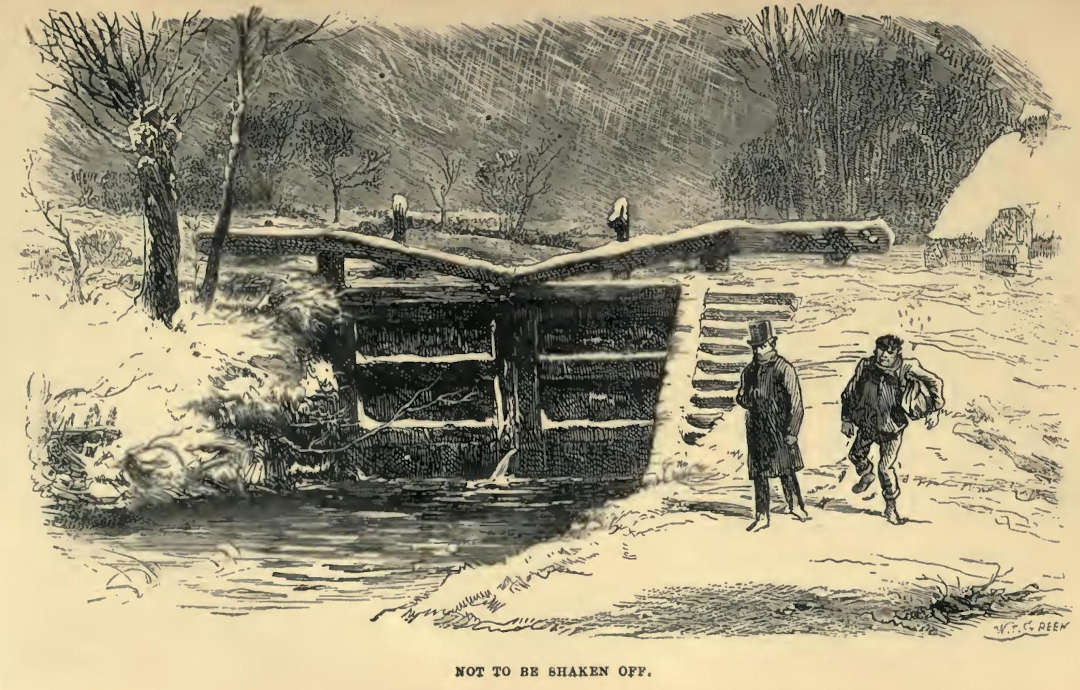
\includegraphics[scale=2.3]{04-15-01}

‘Come, come, Master,’ urged Riderhood, at his side. ‘This is a dry game.
And where’s the good of it? You can’t get rid of me, except by coming to
a settlement. I am a going along with you wherever you go.’

Without a word of reply, Bradley passed quickly from him over the wooden
bridge on the lock gates. ‘Why, there’s even less sense in this move
than t’other,’ said Riderhood, following. ‘The Weir’s there, and you’ll
have to come back, you know.’

Without taking the least notice, Bradley leaned his body against a post,
in a resting attitude, and there rested with his eyes cast down. ‘Being
brought here,’ said Riderhood, gruffly, ‘I’ll turn it to some use by
changing my gates.’ With a rattle and a rush of water, he then swung-to
the lock gates that were standing open, before opening the others. So,
both sets of gates were, for the moment, closed.

‘You’d better by far be reasonable, Bradley Headstone, Master,’ said
Riderhood, passing him, ‘or I’ll drain you all the dryer for it, when we
do settle.--Ah! Would you!’

Bradley had caught him round the body. He seemed to be girdled with an
iron ring. They were on the brink of the Lock, about midway between the
two sets of gates.

‘Let go!’ said Riderhood, ‘or I’ll get my knife out and slash you
wherever I can cut you. Let go!’

Bradley was drawing to the Lock-edge. Riderhood was drawing away from
it. It was a strong grapple, and a fierce struggle, arm and leg. Bradley
got him round, with his back to the Lock, and still worked him backward.

‘Let go!’ said Riderhood. ‘Stop! What are you trying at? You can’t drown
Me. Ain’t I told you that the man as has come through drowning can never
be drowned? I can’t be drowned.’

‘I can be!’ returned Bradley, in a desperate, clenched voice. ‘I am
resolved to be. I’ll hold you living, and I’ll hold you dead. Come
down!’

Riderhood went over into the smooth pit, backward, and Bradley Headstone
upon him. When the two were found, lying under the ooze and scum behind
one of the rotting gates, Riderhood’s hold had relaxed, probably in
falling, and his eyes were staring upward. But, he was girdled still
with Bradley’s iron ring, and the rivets of the iron ring held tight.



